\documentclass[border=10pt]{standalone}
\usepackage{tikz}
\usetikzlibrary{trees, positioning, fit, calc, shadows}
\usepackage{helvet}
\renewcommand{\familydefault}{\sfdefault}

\begin{document}
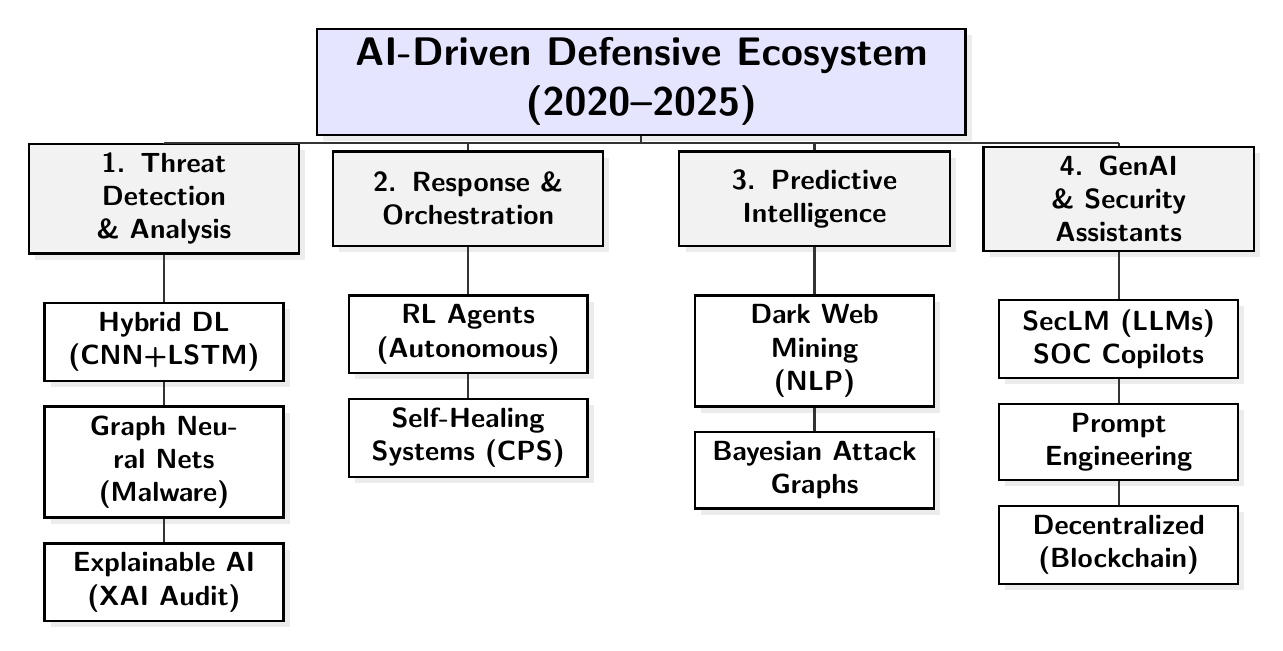
\begin{tikzpicture}[
    node distance=0.4cm,
    font=\bfseries, % Fonte negrito
    % Estilos
    box/.style={
        draw, rectangle, fill=white, align=center, 
        minimum height=0.8cm, text width=2.8cm, 
        drop shadow={opacity=0.15}, line width=0.8pt
    },
    % --- AJUSTE AQUI: Aumentei a largura para 8cm ---
    root_box/.style={
        box, fill=blue!10, text width=8cm, 
        minimum height=1.2cm, font=\Large\bfseries
    },
    cat_box/.style={
        box, fill=gray!10, text width=3.2cm, 
        minimum height=1.2cm
    },
    line/.style={-, thick, color=black!80}
]

    % --- NÓS ---
    \node[root_box] (root) {AI-Driven Defensive Ecosystem\\(2020--2025)};
    
    % Coordenada auxiliar para alinhar a fileira de baixo
    \coordinate[below=0.8cm of root] (aux_row1);
    
    % Categorias (Nível 1)
    % Usamos a coordenada auxiliar para garantir alinhamento perfeito
    % \node[cat_box] (c2) at (aux_row1 -| root.west) {2. Response \&\\Orchestration}; 
    % Nota: Ajustei a posição relativa do C2 para alinhar melhor com a nova largura
    % Mas manter o alinhamento relativo ao centro funciona melhor:
    
    % Vamos reposicionar as categorias baseadas no centro para ficar simétrico com a raiz larga
    \node[cat_box] (c_center_left) at ([xshift=-2.2cm]aux_row1) {2. Response \&\\Orchestration};
    \node[cat_box] (c_center_right) at ([xshift=2.2cm]aux_row1) {3. Predictive\\Intelligence};
    \node[cat_box, left=0.4cm of c_center_left] (c_left) {1. Threat Detection\\\& Analysis};
    \node[cat_box, right=0.4cm of c_center_right] (c_right) {4. GenAI \& Security\\Assistants};

    % Renomeando para facilitar o resto do código (c1, c2, c3, c4)
    \coordinate (c1) at (c_left);   
    \coordinate (c2) at (c_center_left);
    \coordinate (c3) at (c_center_right);
    \coordinate (c4) at (c_right);

    % Folhas C1
    \node[box, below=0.6cm of c_left] (l1a) {Hybrid DL\\(CNN+LSTM)};
    \node[box, below=0.3cm of l1a] (l1b) {Graph Neural Nets\\(Malware)};
    \node[box, below=0.3cm of l1b] (l1c) {Explainable AI\\(XAI Audit)};
    
    % Folhas C2
    \node[box, below=0.6cm of c_center_left] (l2a) {RL Agents\\(Autonomous)};
    \node[box, below=0.3cm of l2a] (l2b) {Self-Healing\\Systems (CPS)};
    
    % Folhas C3
    \node[box, below=0.6cm of c_center_right] (l3a) {Dark Web Mining\\(NLP)};
    \node[box, below=0.3cm of l3a] (l3b) {Bayesian Attack\\Graphs};
    
    % Folhas C4
    \node[box, below=0.6cm of c_right] (l4a) {SecLM (LLMs)\\SOC Copilots};
    \node[box, below=0.3cm of l4a] (l4b) {Prompt\\Engineering};
    \node[box, below=0.3cm of l4b] (l4c) {Decentralized\\(Blockchain)};

    % --- CONEXÕES ---
    
    % Linha Vertical da Raiz
    % Calculamos o ponto médio entre as categorias centrais para descer a linha
    \path (c_center_left.east) -- (c_center_right.west) coordinate[midway] (center_point);
    \path (root.south) -- (center_point |- c_center_left.north) coordinate[midway] (bus_y);
    
    \draw[line] (root.south) -- (root.south |- bus_y);

    % Barra Horizontal (Bus)
    \draw[line] (c_left.north |- bus_y) -- (c_right.north |- bus_y);

    % Pernas Verticais para Categorias
    \draw[line] (c_left.north |- bus_y) -- (c_left.north);
    \draw[line] (c_center_left.north |- bus_y) -- (c_center_left.north);
    \draw[line] (c_center_right.north |- bus_y) -- (c_center_right.north);
    \draw[line] (c_right.north |- bus_y) -- (c_right.north);

    % Cadeias (Pai -> Filho)
    \draw[line] (c_left.south) -- (l1a.north); \draw[line] (l1a.south) -- (l1b.north); \draw[line] (l1b.south) -- (l1c.north);
    \draw[line] (c_center_left.south) -- (l2a.north); \draw[line] (l2a.south) -- (l2b.north);
    \draw[line] (c_center_right.south) -- (l3a.north); \draw[line] (l3a.south) -- (l3b.north);
    \draw[line] (c_right.south) -- (l4a.north); \draw[line] (l4a.south) -- (l4b.north); \draw[line] (l4b.south) -- (l4c.north);

\end{tikzpicture}
\end{document}